\section{Building the Visualization}\label{sec:dev}
In this section I turn to the development of the visualization website. In \autoref{sec:dev-data} I describe the process of collecting and cleaning the data used; \autoref{sec:dev-sketches} and \autoref{sec:dev-wireframes} present the design and testing of the early, low-fidelity designs for the site. The development of the website itself is described in \autoref{sec:dev-website}, and \autoref{sec:dev-testing} discusses the results of testing the website with members of its intended audience.

\subsection{Data Collection \& Cleaning}\label{sec:dev-data}
As discussed in \autoref{sec:design-data}, I used AP exam data from the College Board\footnote{AP Demographics available at \url{https://research.collegeboard.org/programs/ap/data}}, graduation data from the Taulbee Survey\footnote{Taulbee Survey available at \url{http://cra.org/resources/taulbee-survey/}}, and employment data from the U.S. Bureau of Labor Statistics\footnote{Labor Statistics available at \url{https://www.bls.gov/cps/tables.htm}}
 to construct the visualizations. \autoref{tbl:data-sources} summarizes the subset of each dataset used for this project.

\begin{table}
  \begin{tabular}{L{3.6cm}cL{4cm}l} \hline
    \textbf{Data Source} & \textbf{Years Included} & \textbf{Subset} & \textbf{Variables} \\ \hline
    \href{https://research.collegeboard.org/programs/ap/data}{College Board AP Demographics}
      & 2010--2016
      & AP Computer Science Exam
      & Gender, Exam Score \\
    \href{http://cra.org/resources/taulbee-survey/}{CRA's Taulbee Survey}
      & 2010--2015
      & Graduate \& Undergraduate degrees awarded
      & Gender, Program \\
    \href{https://www.bls.gov/cps/tables.htm}{United States Bureau of Labor Statistics Detailed Employment (Table 11)}
      & 2011--2015
      & Computing Occupations
      & Gender, Occupation \\ \hline
  \end{tabular}
  \caption{Summary of Data Sources Used}\label{tbl:data-sources}
\end{table}

Where feasible, I collected all data going back to 2010; the Bureau of Labor Statistics changed their reporting categories in 2011, so for consistency I excluded their 2010 data. Only the College Board had released 2016 data at the time of collection. Because not all groups contain the same years' data, visualizations including multiple groups use percentage breakdowns by gender, rather than absolute numerical comparisons.

All three data sources are available either as spreadsheets or in PDF tables. The College Board spreadsheets include demographic information for all AP tests, broken out by gender and by exam score, so I extracted the data for the Computer Science exam and discarded the others. The Bureau of Labor Statistics similarly includes all occupations in their spreadsheet, so I extracted the data for all of the ``Computer and Mathematical Occupations'' as seen in the literature. The Taulbee Survey publishes its data as part of an annual PDF report; because the data is already aggregated (and consequently fairly small), I manually copied the data from their PDFs into a CSV file.

Both the College Board and the Taulbee Survey give the aggregated counts of male and female students for each relevant category, so the only further processing required was to format each row consistently. The Bureau of Labor Statistics, on the other hand, provides a total count of employees for each category, rounded to the nearest thousand, along with the percentage of women employed in each category. They do not provide diversity statistics for categories with fewer than 50,000 total employees, so I excluded these categories from the visualization. For the categories included, I used the percentages of female employees to calculate an approximate female employee count, to better correspond with the data for educational stages.

\subsection{Early Design Sketches}\label{sec:dev-sketches}
\begin{figure}
  \centering
  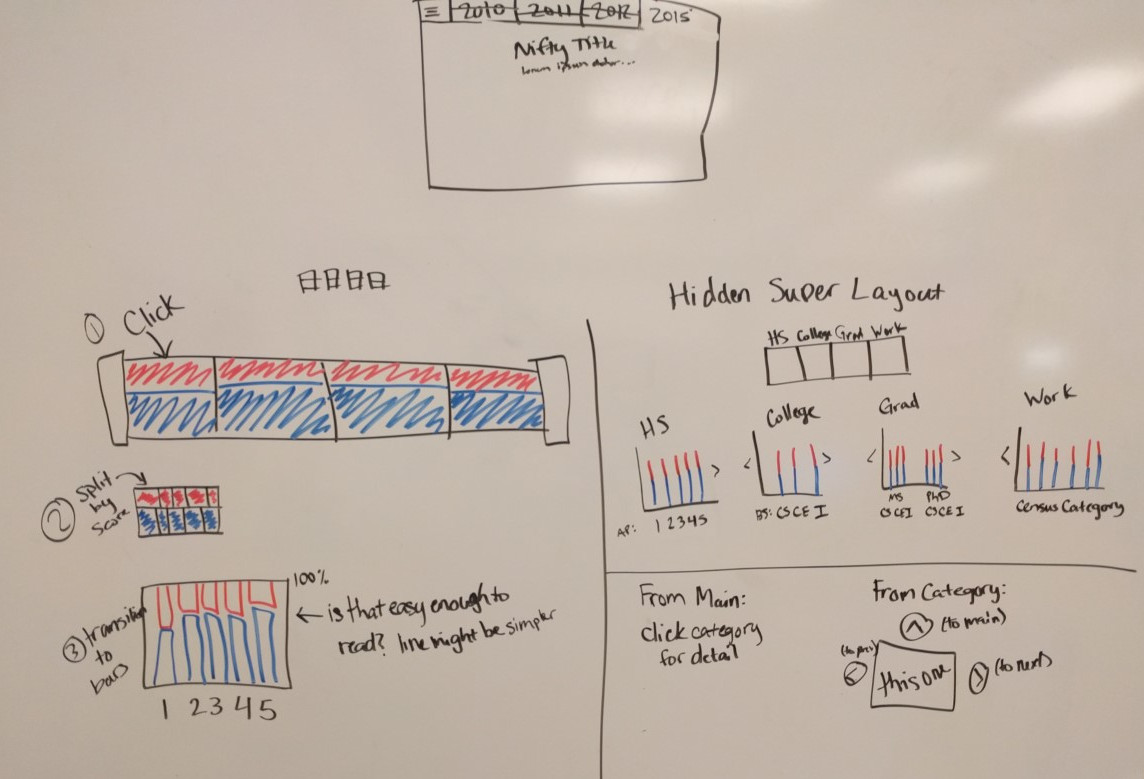
\includegraphics[width=0.8\textwidth]{whiteboard-1-layout}

  \vspace{0.1in}

  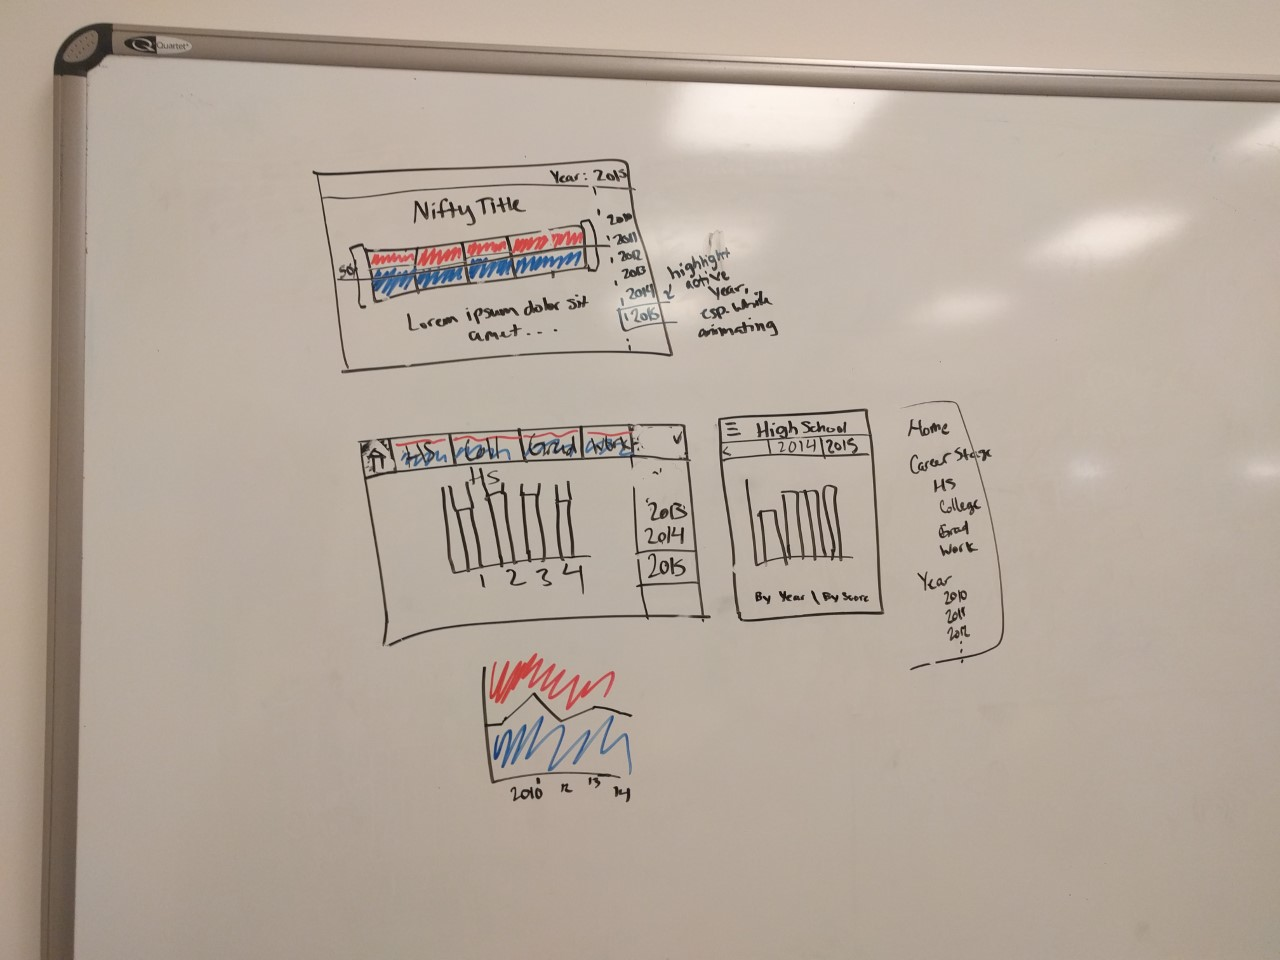
\includegraphics[width=0.8\textwidth]{whiteboard-2-navigation}
  \caption{Early Design Sketches: page layout (top) and alternate navigation (bottom)}\label{fig:whiteboard}
\end{figure}

I used low-fidelity whiteboard sketches to design and test early versions of the webpage before creating a code version. In the early designs, shown in \autoref{fig:whiteboard}, I focused on the visual relationship between the overview and the detailed views of each pipeline stage, on page navigation, and on graph types to display data. The top sketch shows disassembled overview of the page layout. The page frame at the top of the sketch uses a top navigation based on the stages of the tech education pipeline, so users interested in a particular stage can jump directly to it. To the left, it uses a pipe segment to visually represent the pipeline, which is divided into sections and color-coded according to the gender ratio of that section. The numbered sections below the pipe model a proposed animation from the overview into a bar graph for one of the detailed views. The right panel shows the spatial relationship between views, with vertical movement from the overview to each detailed view and horizontal movement between stages of the pipeline. This was intended to use the chronological nature of the pipeline to suggest a narrative on its own, connecting one stage of the pipeline to the next in the same way an individual would follow them throughout her career.

However, truly following the flow of a single career would require longitudinal data, which the combination of aggregated datasets cannot provide. Instead, the data supports viewing trends over time, so the bottom sketch explores ways to include time series information in the page navigation. The first panel introduces a drop-down menu to filter the entire display by year, with an option to animate through all available years. The next displays show alternatives for desktop and mobile views: on a large display, the top menu gets a series of colored backgrounds to mimic the color-coding of the overview pipe, with the same year filter as a dropdown. On smaller displays, the menu collapses into a hamburger pullout, and the year filter is present both within that menu and directly under the header, where it can be swiped sideways as needed. The bottom frame shows a color-coded area chart tracking the gender ratio over time.

The smudges in \autoref{fig:whiteboard} are evidence of my first round of testing, intended to determine whether the time-based navigation would make sense to viewers. Since this was a very preliminary test, I did not use rigorous standards for selecting participants or testing the layout: I asked nearby classmates who had no familiarity with my design goals if they would exchange feedback for a cookie. Two volunteered, so I brought them one at a time to the whiteboard, gave them a one-sentence introduction to the purpose of the site, and asked how they would interact with it. As they explained (or ``clicked'' on the whiteboard), I drew in details or menus, as needed.

Only one of the two found the drop-down without prompting, and she said she was unlikely to use a filter placed that far away from the graphs it applied to. The other participant simply wanted to scroll for more information.

\subsection{Refined Design Wireframes}\label{sec:dev-wireframes}
\begin{figure}
  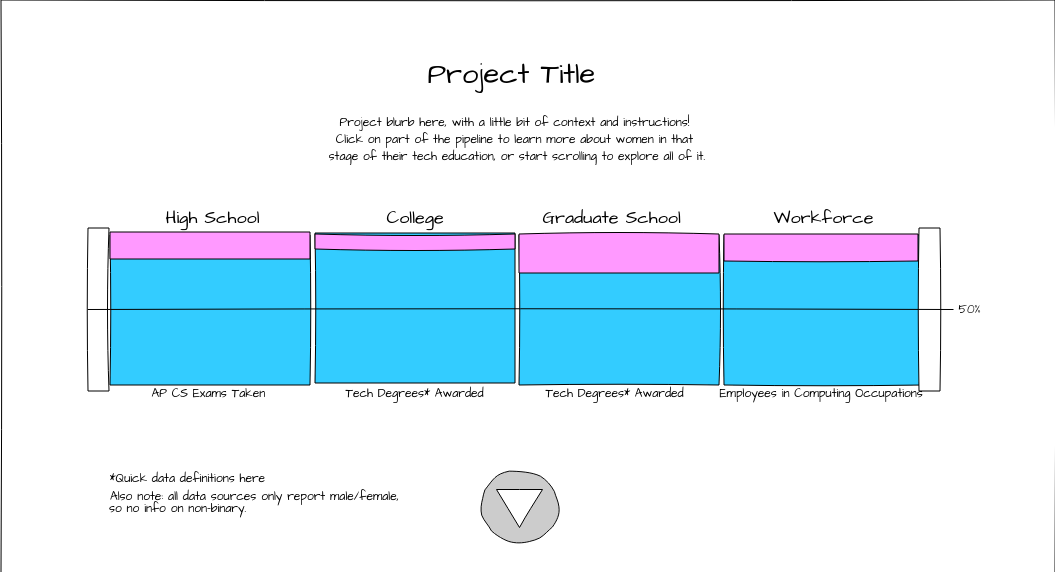
\includegraphics[width=\textwidth]{wireframe-1-overview}

  \vspace{2cm}

  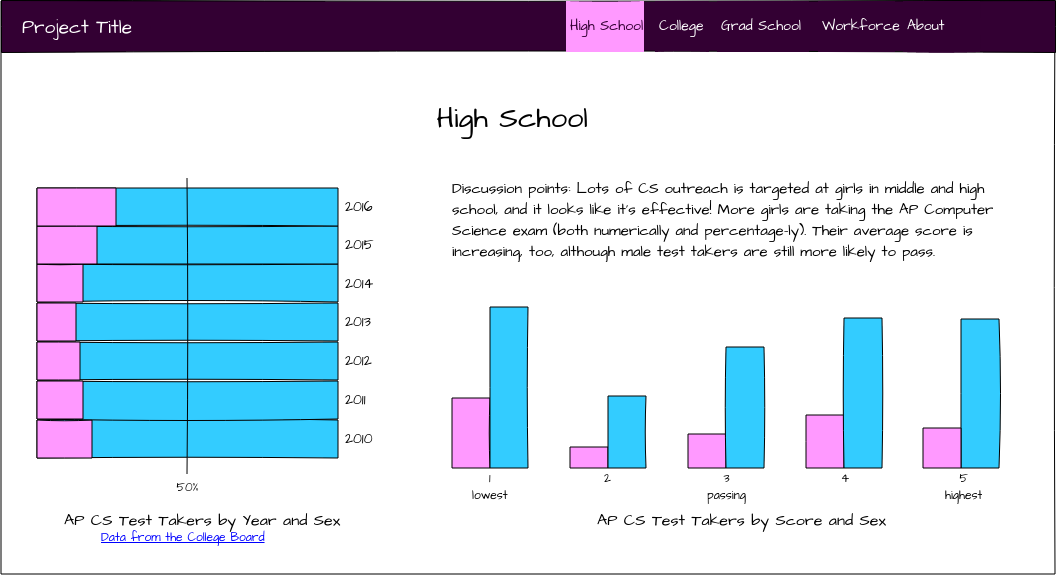
\includegraphics[width=\textwidth]{wireframe-2-hs-detail}
  \caption{Wireframes: overview (top) and high school detail (bottom)}\label{fig:wireframes}
\end{figure}

Since neither test participant found the time-based navigation useful, I removed it and simplified the page navigation for the next iteration of the design. Instead of a menu, viewers see a downward arrow indicating the page is scrollable; in this design, scrolling takes users from the overview to the detailed views, as well as from one detailed view to the next.

I also added narrative descriptions to each detailed view, to discuss issues unique to that stage in the pipeline and to highlight data of interest within that stage. This provides the context necessary to understand the data, with both background information to help viewers build a mental model of the overall pipeline and guidance on how to interpret this specific data. I separated time series data and data by group (AP score, academic program, or specialized occupation) into two separate graphs, placed side-by-side, to show both the granular group data and the trends over time without relying on another menu. \autoref{fig:wireframes} shows the wireframes produced at the end of this refinement, made with the Pencil Prototyping tool\footnote{\url{http://pencil.evolus.vn/Next.html}}.

I performed another casual test at this point in the process, recruiting two new testers who roughly fit the personas presented in \autoref{sec:design-users}: a classmate interested in web development to represent Laurie's opinion, and an undergraduate communications major to represent Gabriella's. In addition to verifying that the simpler navigation was easier to understand, I used this test to compare ways of presenting the narrative elements. After explaining how they would interact with a page containing only the graphs and headings, they saw three different versions of the page: the same graphs-only layout, one with introductory text for each section, and one with annotations added to interesting points on the graph. The introductory texts were written on sticky notes and the annotations were on Post-It flags, so the two test layouts were of similar quality. Both testers preferred the version with introductory text pictured in the final wireframes, claiming the original version needed more explanation but that the annotations distracted from the graphs.


\subsection{Website Development}\label{sec:dev-website}
\begin{figure}
  \begin{minipage}{0.49\textwidth}
    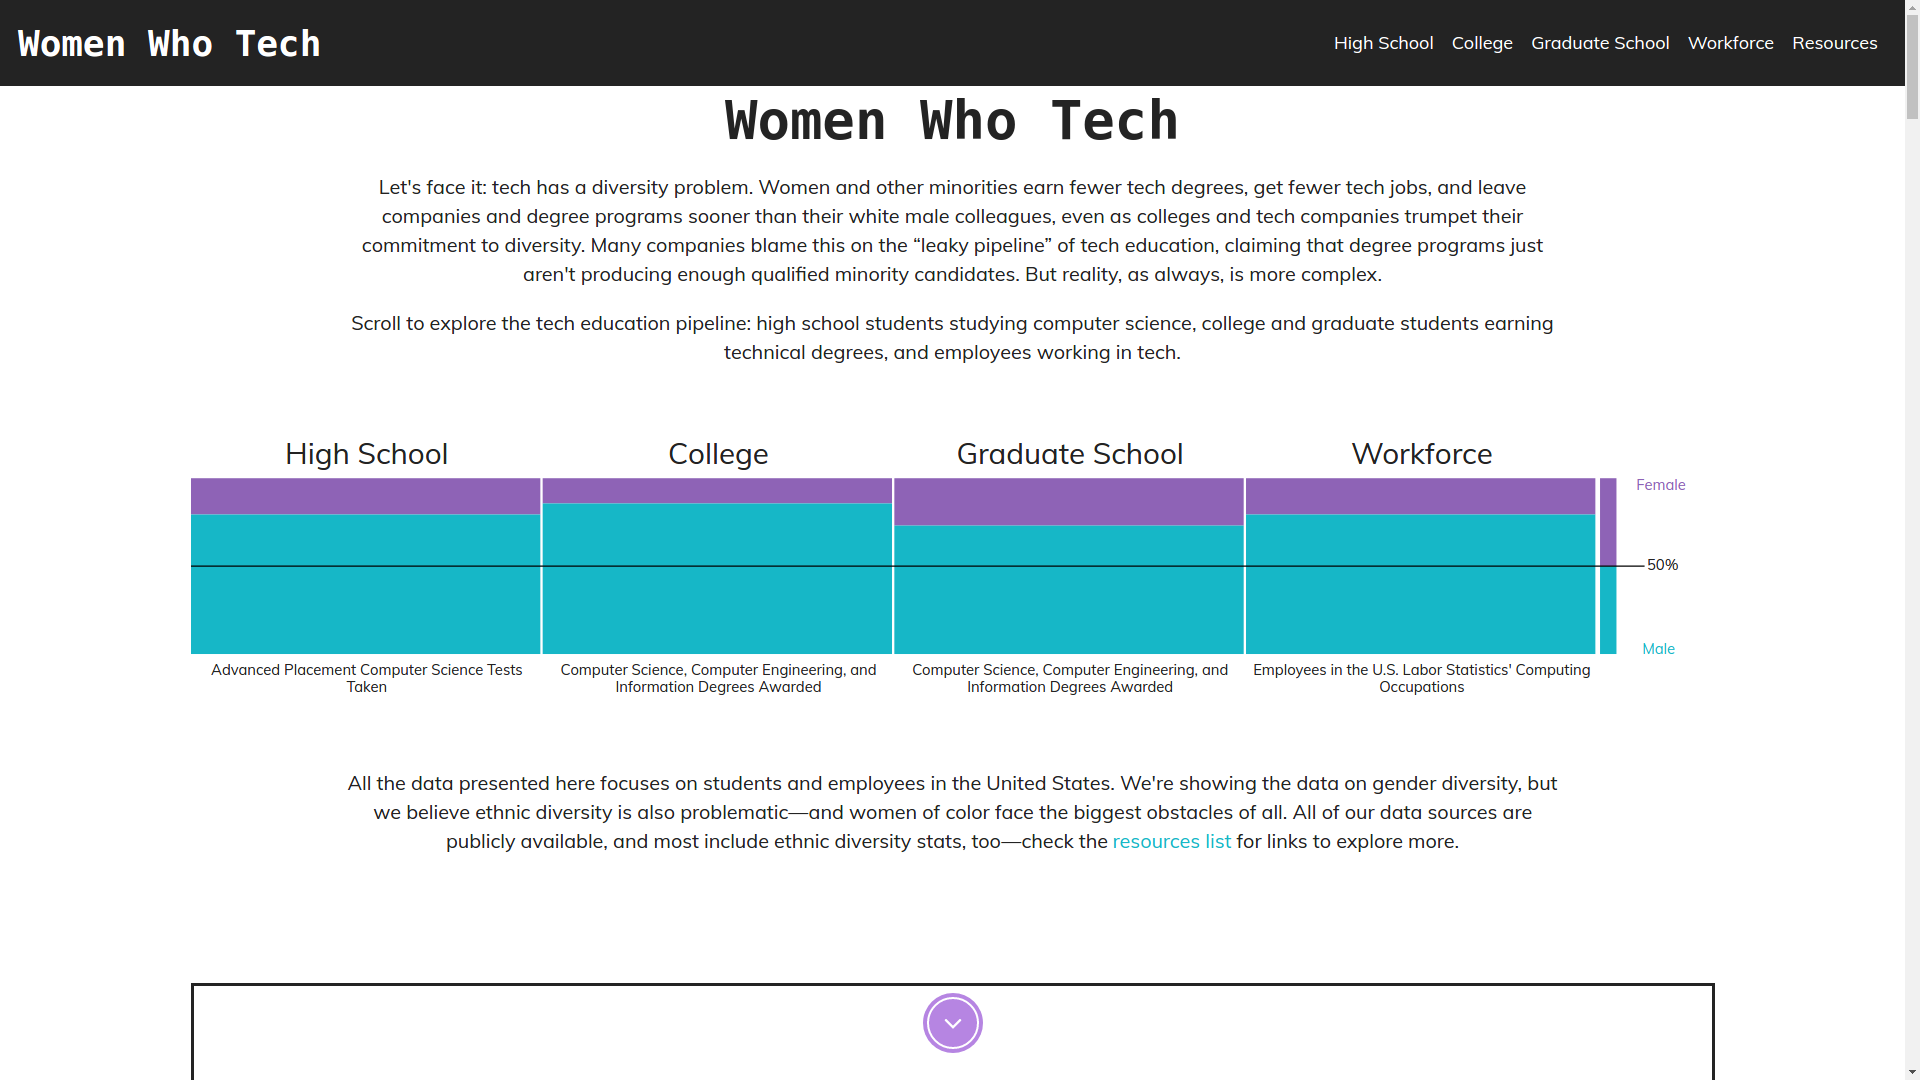
\includegraphics[width=\textwidth]{screen-1-overview}
    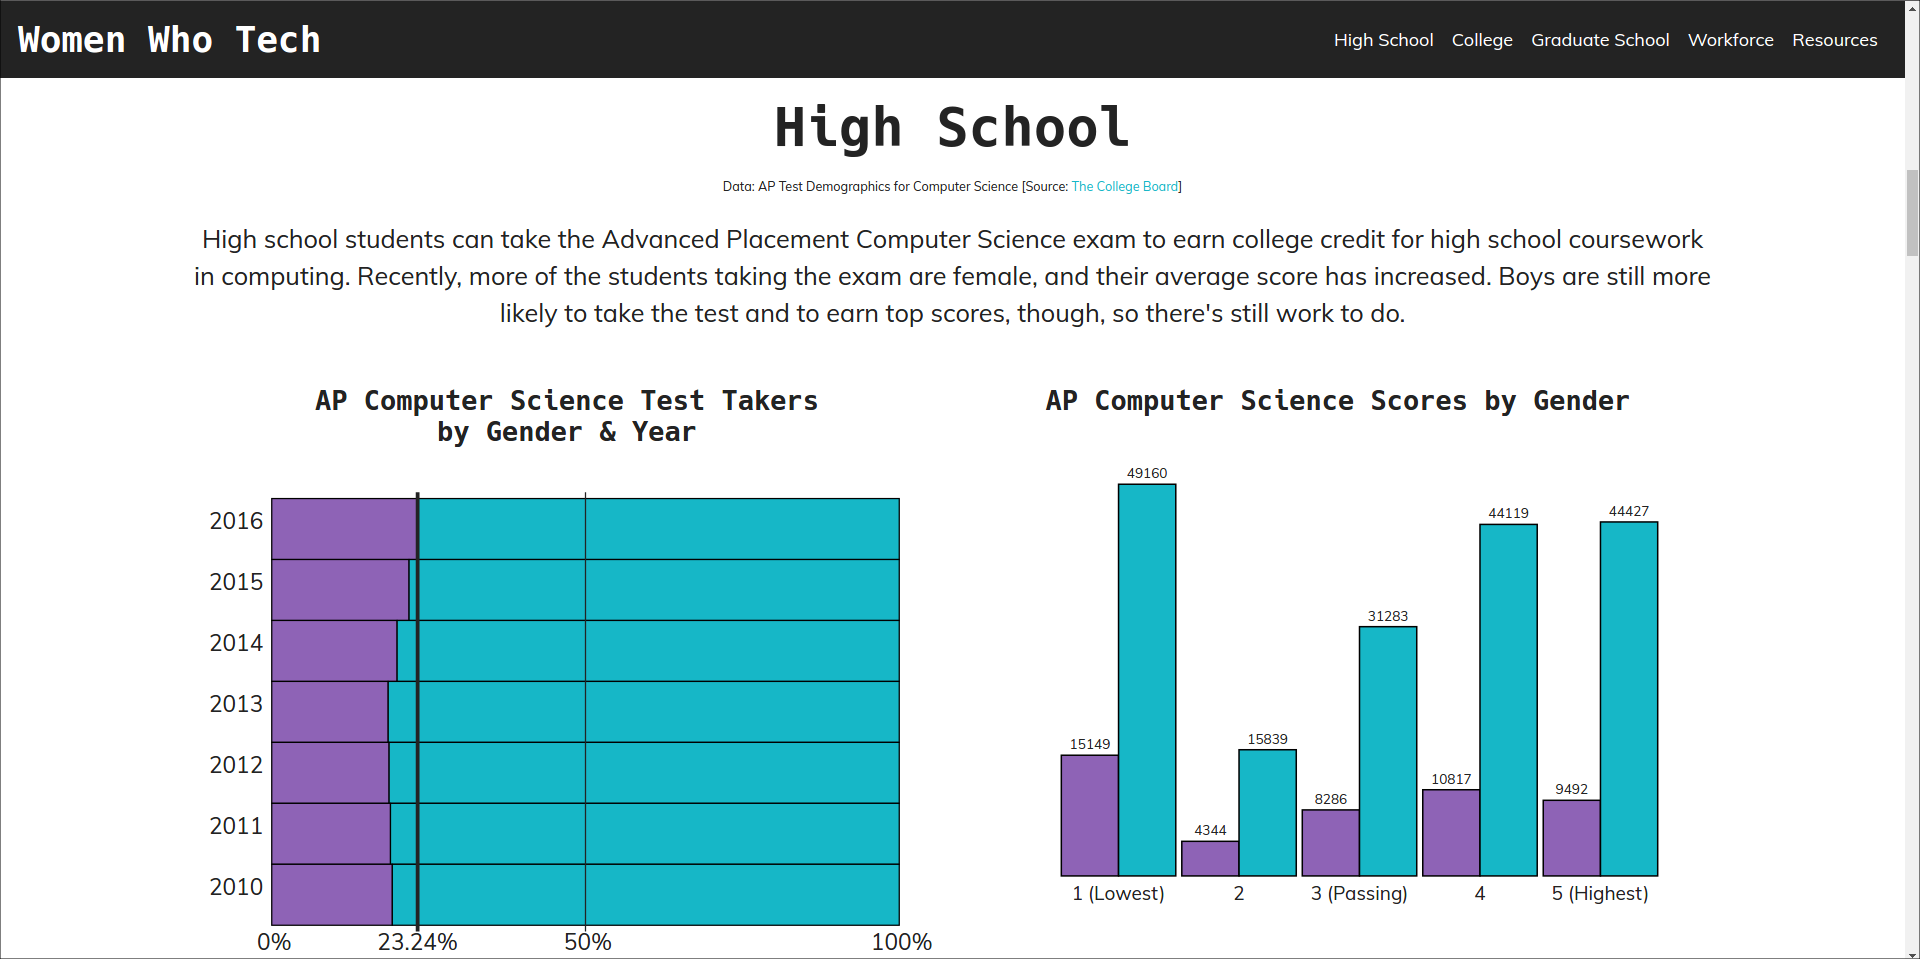
\includegraphics[width=\textwidth]{screen-3-hs-detail}
  \end{minipage}
  \begin{minipage}{0.49\textwidth}
    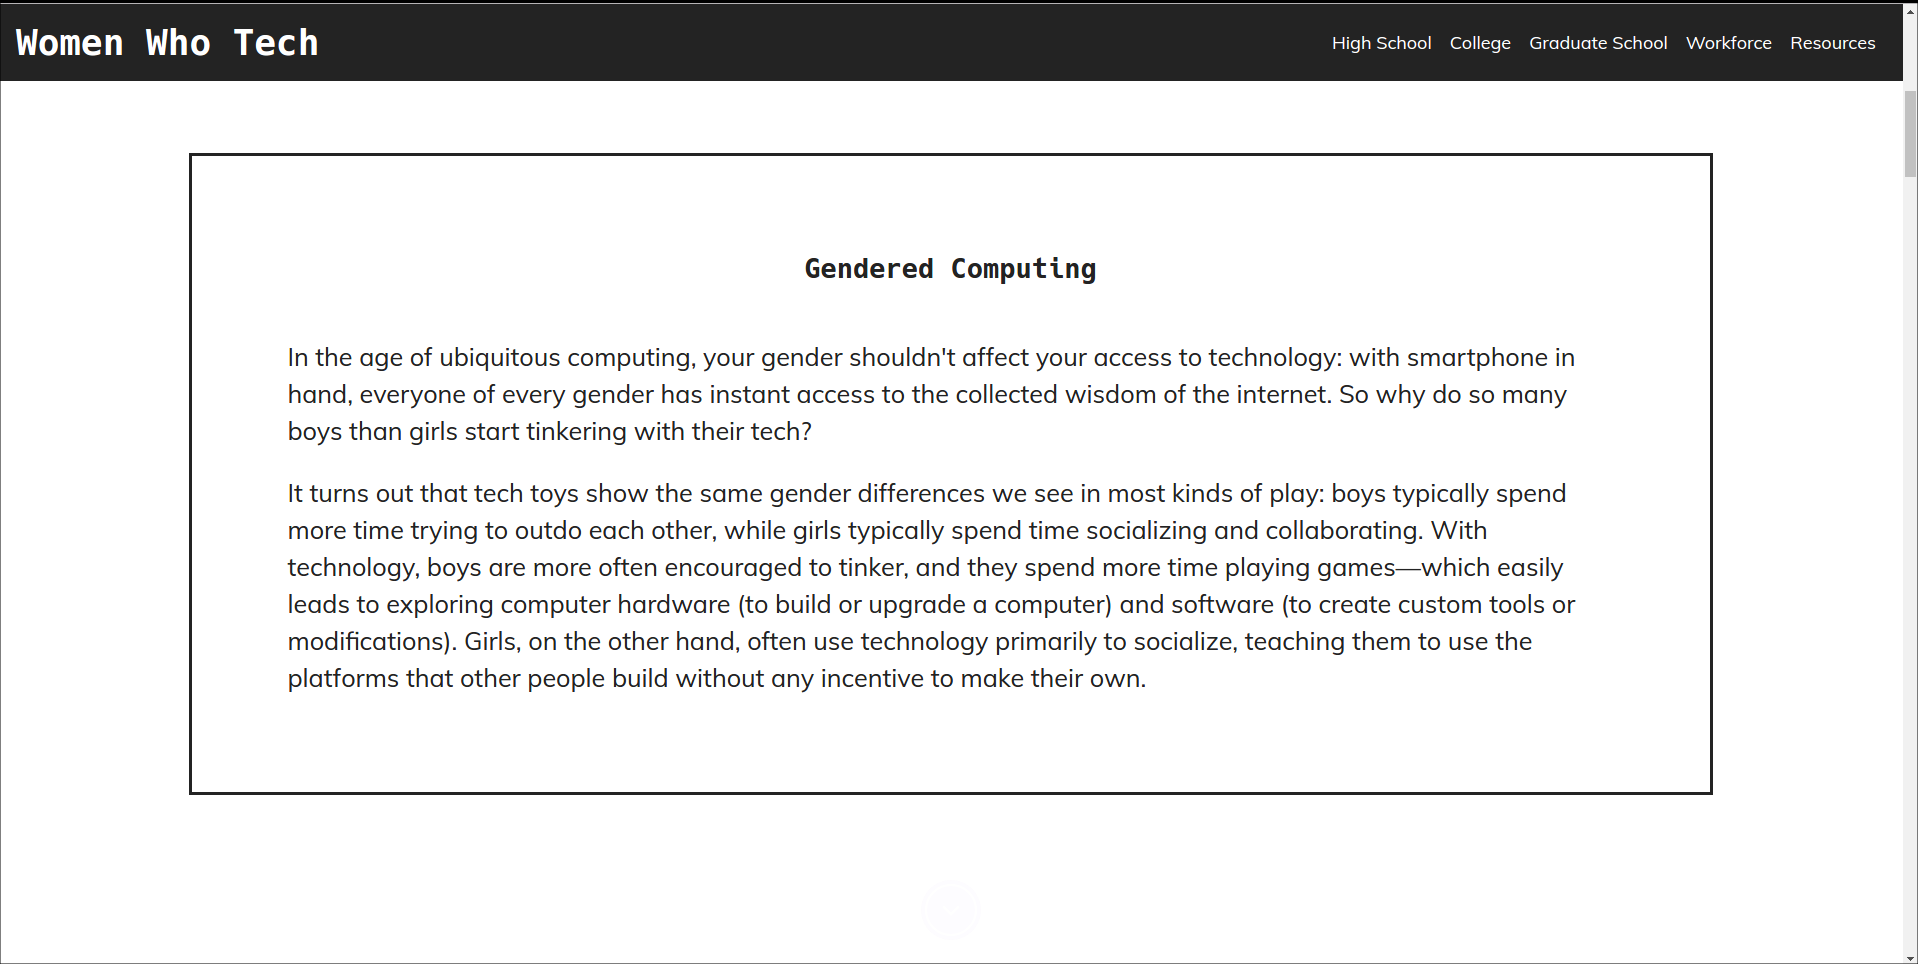
\includegraphics[width=\textwidth]{screen-2-interlude}
    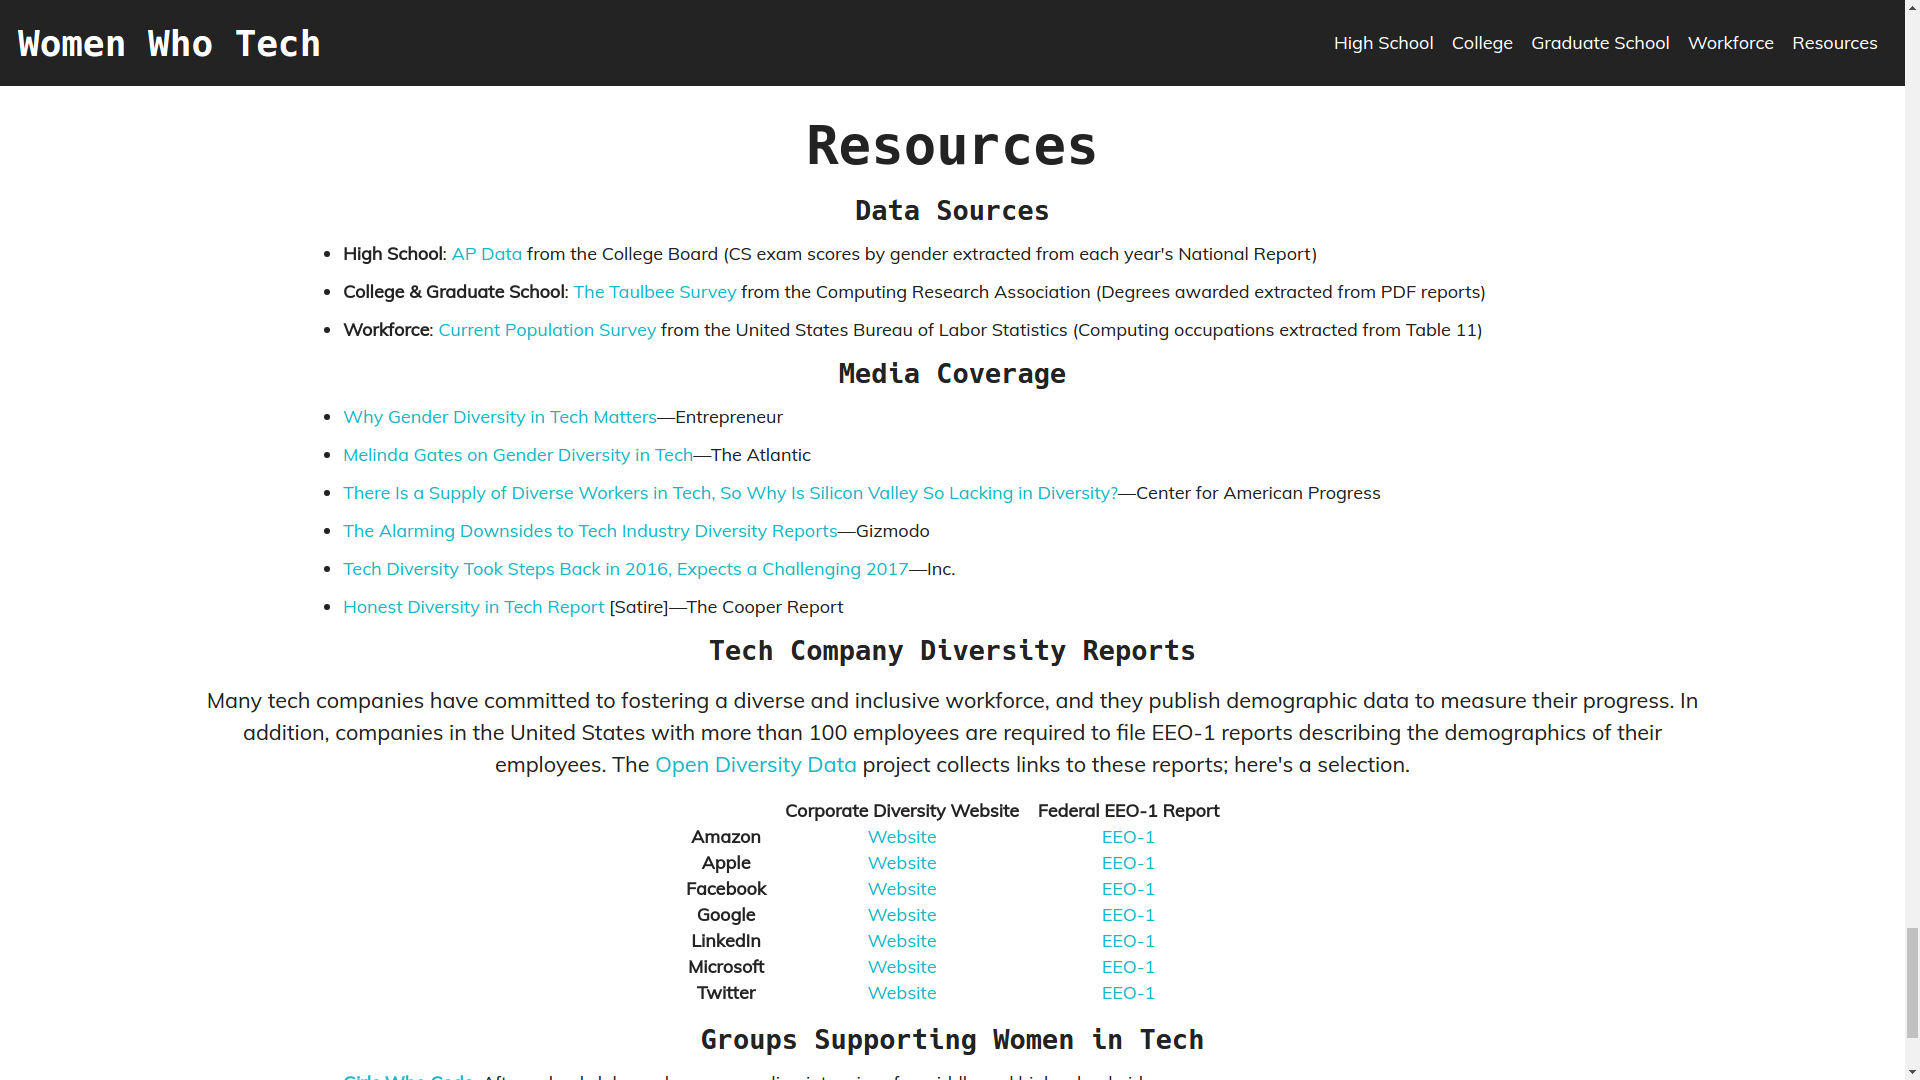
\includegraphics[width=\textwidth]{screen-11-resources}
  \end{minipage}
  \caption{Schematic Screenshots: pipeline overview (top left), narrative frame (top right), high school detail (bottom left), resources (bottom right). The remainder of the page repeats the basic layout of the narrative frame and detail view.}\label{fig:screenshots}
\end{figure}

After testing the wireframes, I began constructing the website itself using HTML5/CSS3 for the page layout and the D3.js JavaScript library\footnote{\url{https://d3js.org/}} for the visualizations. The website is available online, with a link to the source code, at \url{https://thekatheri.net/tech-ladies/}. The screenshots in \autoref{fig:screenshots} show the layouts used in the webpage, from left to right according to their order on the website. The layout is responsive, resizing both the text areas and the visualizations to accommodate smaller screens. This ensures the page is viewable on any device, although at this time only the textual portions are accessible to non-visual devices like screenreaders.

The overview panel, in the top right, contains the pipeline visualization used in the wireframes, with a color legend to the right of the pipeline. The pipeline visualization shows the ratio of men to women in each pipeline stage throughout all years in the dataset, providing a broad picture of the continuing lack of gender diversity in tech. It includes a 50\% line for reference. The overview is immediately preceded by instructions to scroll for more details and is followed by a downward arrow, so that viewers can examine the overview but also know how to access the details as desired. A navigation bar is always present at the top of the page, so viewers who want to jump directly between states can do so at any time.

The overview is followed by the first of several narrative panels, pictured in the top left of \autoref{fig:screenshots}. These are framed boxes with one to three short paragraphs presenting relevant background from the academic literature or suggestions to improve gender diversity at a particular stage in the pipeline.

A narrative panel precedes each detailed view, like the high school panel in the bottom right of \autoref{fig:screenshots}. The detailed views begin with a link to the data source for that stage, include an introductory paragraph summarizing the data and identifying a point of interest, and present the two graphs by year and by category side-by-side (on wide screens) or one after the other (on smaller screens). While only the high school view is pictured, all detailed views currently use the same layout.

At the end of the page, after the detailed view of the workforce data, is a resources list. This includes links to the datasets used with information about the subset included, so that others can extract the same data if they choose to; a selection of media articles about diversity in tech; links to several large tech companies' diversity websites and Equal Employment Opportunity reports; and several nonprofit and professional organizations that support women and girls developing or pursuing an interest in technology.

\begin{figure}
  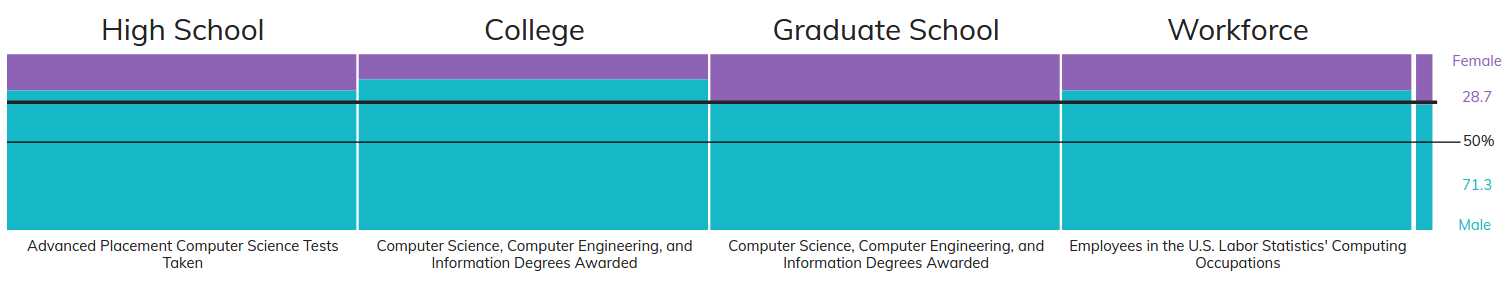
\includegraphics[width=0.95\textwidth]{screen-12-overview-interaction}

  \begin{minipage}{0.5\textwidth}
    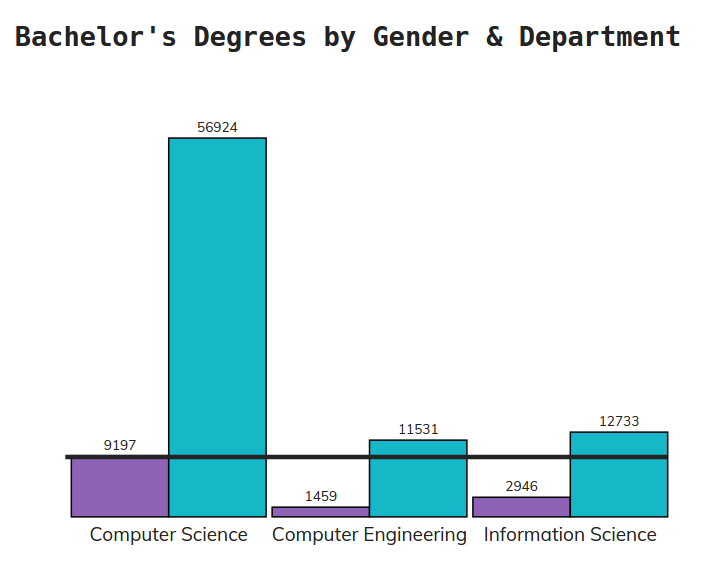
\includegraphics[width=0.95\textwidth]{screen-13-category-interaction}
  \end{minipage}
  \begin{minipage}{0.5\textwidth}
    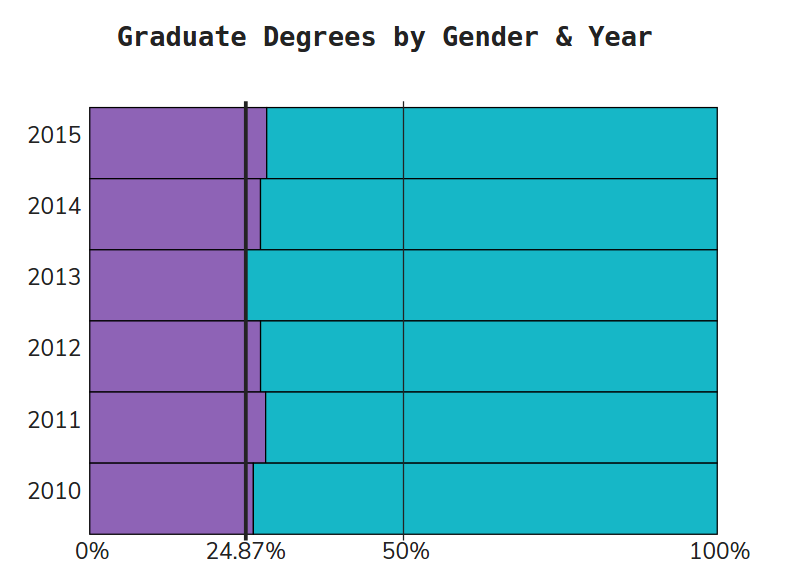
\includegraphics[width=0.95\textwidth]{screen-14-year-interaction}
  \end{minipage}
  \caption{Graph Interactions: gender breakdown on the overview (top), reference line on details by group (bottom left), reference line with percent female on details by year (bottom right)}\label{fig:interactions}
\end{figure}

Each visualization also contains hover interactions as a progressive enhancement to allow desktop and laptop users to explore the data more precisely. \autoref{fig:interactions} shows the interaction for each graph type. In all three cases, the primary goal is to provide a way for users to compare values across graphs that are potentially quite tall or wide; for consistency, all three use a thick black line to mark the position of interest. In the overview, pictured at the top of \autoref{fig:interactions}, this line follows the user's mouse and adjusts both the visual and numerical percentages displayed in the legend to the right. The graphs that show gender by category (degree, pictured bottom left, or AP score or occupation, as appropriate) simply displays a line that follows the user's mouse up and down as a reference point for the rest of the bars in the graph. The line in each graph by year (bottom right) snaps to the percentage of women in the data for the year under the user's mouse to display the percentage more precisely.

\subsection{Testing the Website}\label{sec:dev-testing}
I did two rounds of testing on the website itself: one after coding just the basic layout with placeholder graphs, and one after adding the real graphs, styling the page, and adding the hover interactions. For these later tests, I recruited participants somewhat more carefully and asked more specific questions than when testing the sketches and wireframes; however, all tests were still fairly informal, and none lasted more than about 15 minutes.

Each of these final rounds included four participants, two from each persona. The ``Gabriella'' participants were all students in majors not related to computing; two had basic programming experience, one in SAS and one in simple Java. Neither had any experience with web design or development. The ``Laurie'' participants were all graduate students or young professionals in one of the three fields included in the Taulbee Survey (computer science, computer engineering, or information science). All of these testers have experience with both designing and developing websites, one as a user experience professional designing web components, one in freelance web development, and two through extensive related coursework.

In the first test, I showed testers the prototype webpage and explained that I was primarily looking for feedback on the layout, navigation, and narrative. I asked them to think aloud as they explored the page so I could hear if there were places that needed to be clearer. When they stopped, expressed confusion, or tried to interact with the placeholder graphs, I used prompts like ``What would you expect to be able to do there?'' or ``What questions would you ask if you could talk to the person who did that study?'' to identify their unmet information needs.

For these tests, the detailed view layout matched the wireframes in \autoref{fig:wireframes} rather than the finished layout in \autoref{fig:screenshots}, so all the narrative was in the introductory paragraph to the left of the graph by year. This meant that in some cases, the text was long enough that the two graphs didn't line up, leading to comments like ``I wish I could see both graphs at the same time.'' In other cases, like the view for bachelor's degrees, the text was short enough to preserve alignment, but it did not provide enough information to create a cohesive narrative. One ``Gabriella'' participant commented, ``This is really interesting, but I still don't know how it connects. Why is there such a difference between this graph and the next one?'' Sharing space with the text also caused readability problems on the category graphs; three of the four participants noted that it was hard to see the short bars on the placeholder graphs scaled to fit below the paragraphs. I resolved both of these problems for the next iteration by moving the introduction to its current location above the graphs, and by separating general background information into the narrative frames in between the detailed visualizations.

The earlier test also did not include the scroll arrow, although it appears in both the wireframes and the finished website. This led one participant to navigate entirely using the menu links, which jump directly between visualization sections. While this is a perfectly valid way to navigate the page, with the addition of the narrative frames it would result in missing a significant portion of the page's content. Rather than clutter the menu by adding the extra links, I chose to implement the planned scroll arrow and remove the ability to click on the pipeline to jump to a specific stage. After these changes, all participants successfully navigated through the full narrative.

I followed the same procedure to test the full website, this time asking for general feedback and requesting that testers think aloud as they explored the site. Since the graphs were fully implemented at this point, I also asked questions about the data. Because I wanted to test whether the site successfully allowed participants to explore the things they were interested in, I asked questions about places where they paused or commented, rather than follow the same script for all participants. Since most participants were students (either undergraduate or graduate), this often meant asking about the higher education data. These included questions like ``What year did women earn the most degrees?'' or ``Which degree is the closest to gender-balanced?'' to test whether the graphs were interpretable, as well as questions like ``Why do you think the undergrad and graduate programs are so different?'' to determine whether the narrative text was clear.

All participants answered the probe questions well, although most of them needed the prompt to explore. Their responses to the prompts revealed places for future improvement, summarized in \autoref{tbl:improvements}. The reference line on the category graph (bottom left of \autoref{fig:interactions}) was surprisingly controversial. Two participants commented that they found it distracting and were unsure of its purpose, while one used it extensively to compare across categories. Without any probe questions to prompt it, this participant lined up the reference with the female computer science degrees (as in \autoref{fig:interactions}) and commented, ``This makes me really sad. Computer science is huge, but look! There are fewer girls in computer science than there are boys anywhere else.''

\begin{table}
  \centering

  \begin{tabular}{p{0.9in}p{2.3in}p{2.3in}}\hline
    \textbf{Category} & \textbf{Participant's Comment} & \textbf{Potential Enhancement} \\ \hline
    Interaction (Overview)
      & I wish I could tell exactly where the purple stops.
      & Let the pipe view snap to the data value when the user's mouse nears the boundary \\
    Interaction (Detail)
      & It's hard to tell what group is more balanced. I can tell what has fewer women total, but the ratio is hard to figure out.
      & Add a percentage label to the category graph (possibly on hover, to avoid clutter) \\
    Interaction (Detail)
      & Is there a way to filter the degrees by year?
      & Revive the time-based filtering from the early sketches with simpler controls \\
    Graph Design (Detail)
      & Is there a way to see the total number for a specific year, or is it just the percent?
      & Improve the time series view to show or toggle both the gender ratio and the absolute numbers \\
    Graph Design (Detail)
      & This is interesting information, but the displays all feel the same even though high school and the workforce don't have quite the same problems.
      & Incorporate supplementary datasets to highlight the unique challenges of each stage in the pipeline \\ \hline
  \end{tabular}

  \caption{Test Participant Comments and Future Enhancements}
  \label{tbl:improvements}
\end{table}

Several participants requested more stories, noting that a personal narrative would tie the stages together more cohesively than the background research alone; this cohesion would also help balance the lack of longitudinal data available. Others requested more time-oriented data and a more thorough summary: while all the individual detail views contain time series data, overall trends are never presented together. Additionally, the individual views only show changes in the gender ratio, not in the actual numbers of women (or men) at that stage of the pipeline. Three of the eight testers---one in the first round, two in the second---mentioned that they would like to see a time-based overview, while one of the final testers suggested animating the existing overview. When asked, all four of these participants expressed strong interest in including a timeline that maps the temporal dimension of the data alongside the dates of tech companies' diversity policies, significant nonprofit initiatives, and other related milestones.
